\jxhj{%教学后记
	}
\skrq{%授课日期
	2017年9月21日 4-5节}
\ktmq{%课题名称
	基本指令(二) }
\jxmb{%教学目标,每行前面要加 \item
	\item 掌握G2/G3半径-R的使用;
    \item 掌握G2/G3圆心编程的使用;
    \item 能用G2/G3进行程序的编写;
    \item 掌握编写数控程序的基本思路。}
\jxzd{%教学重点,每行前面要加 \item
	\item G2/G3半径-R的使用;
	\item G2/G3圆心编程的使用;}
\jxnd{%教学难点,每行前面要加 \item
	\item G2/G3圆心编程的使用;}
\jjff{%教学方法
	通过讲述、举例、演示法来说明;}

\makeshouye %制作教案首页

%%%%教学内容
\subsection{组织教学}
\begin{enumerate}[1、]
	\item 集中学生注意力;
	\item 清查学生人数;
	\item 维持课堂纪律;
\end{enumerate}
\subsection{复习导入及主要内容}
\begin{enumerate}[1、]
\item 案例分析;
\item 指令讲解G2/G3;
\item 编写程序;
\item 编写程序的基本思路。
\end{enumerate}

\textbf{案例分析}

在数控铣床或加工中心上加工如图\ref{fig:4-1}所示的零件,试完成程序的编写,已知毛坯为 $\Phi$ 110*30。

\begin{figure}[h]
    \centering
    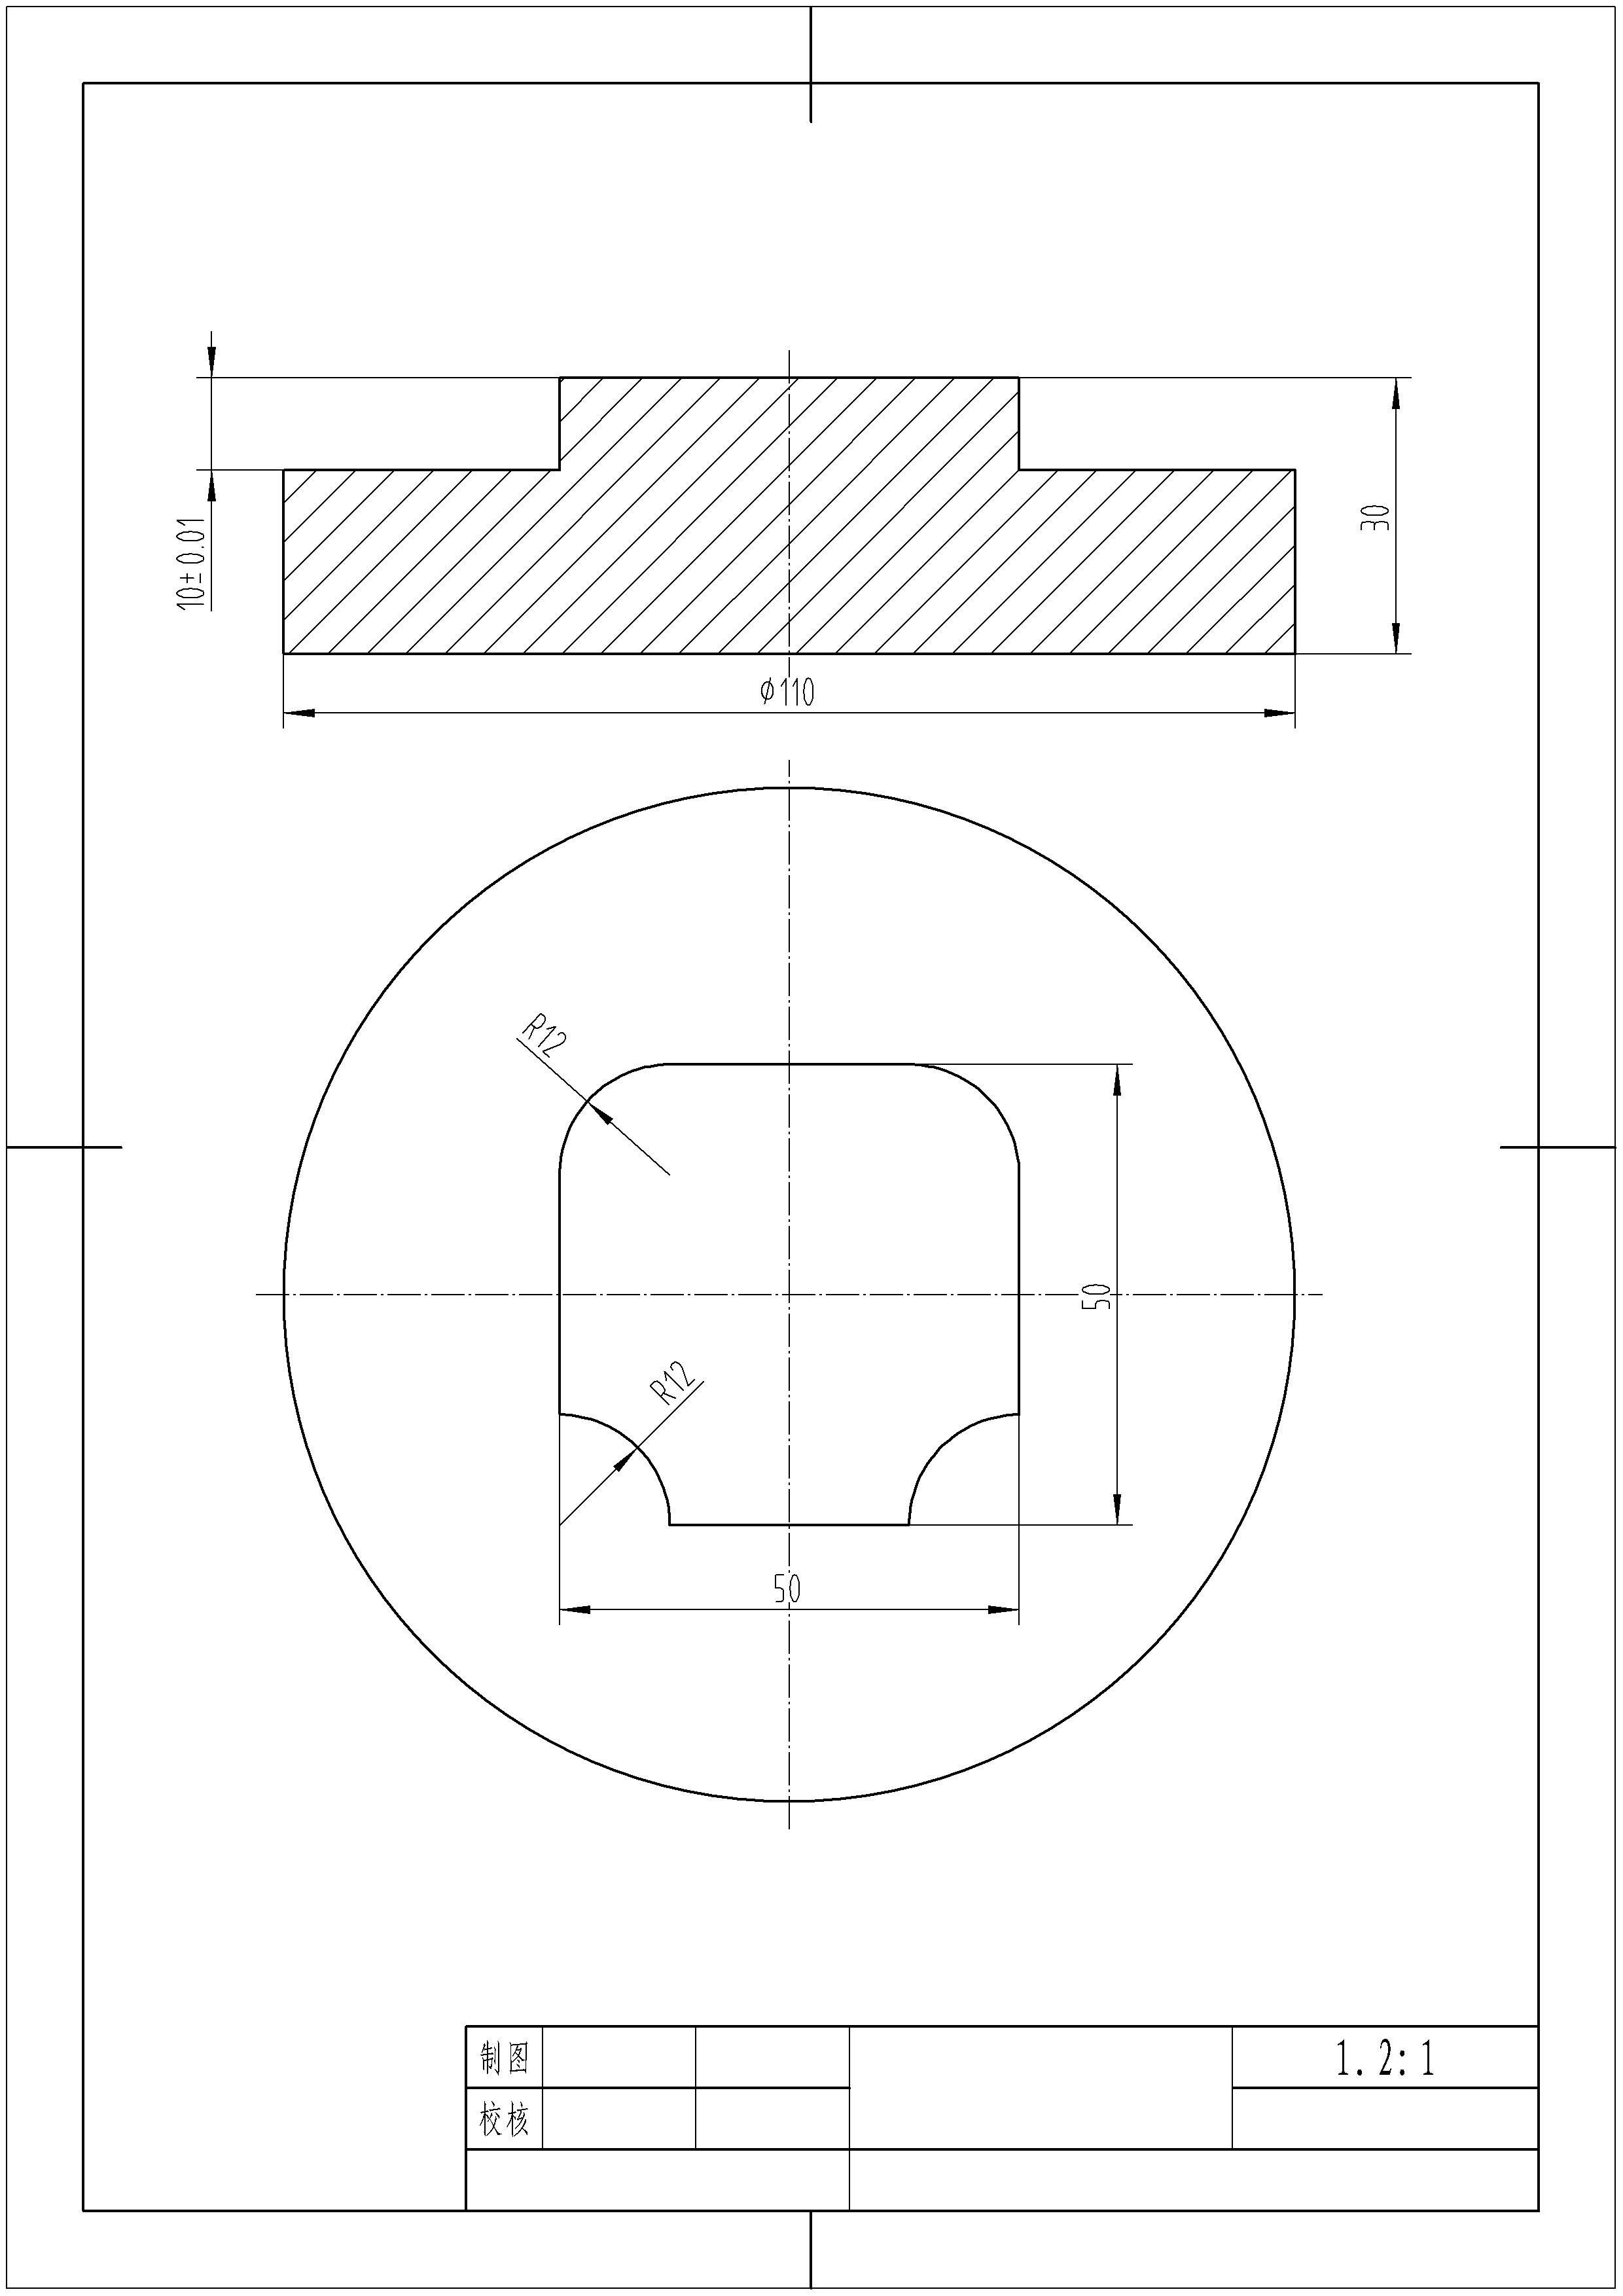
\includegraphics[width=0.8\linewidth,trim=50 150 50 100,clip]{data/image/5-1.jpg}
    \caption{}
    \label{fig:4-1}
\end{figure}

\begin{enumerate}[1、]
    \item 图样分析;
    \item 确定加工内容;
    \item 确定装夹及工件坐标系;
    \item 确定刀具及切削用量;
    \item 确定工序及走刀路线;
    \item 计算点坐标;
    \item 编写程序单。
\end{enumerate}

\subsection{教学内容及过程}

\subsubsection{案例分析}

在数控铣床或加工中心上加工如图\ref{fig:4-1}所示的零件,试完成程序的编写,已知毛坯为 $\Phi$ 110*30。

\begin{figure}[h]
    \centering
    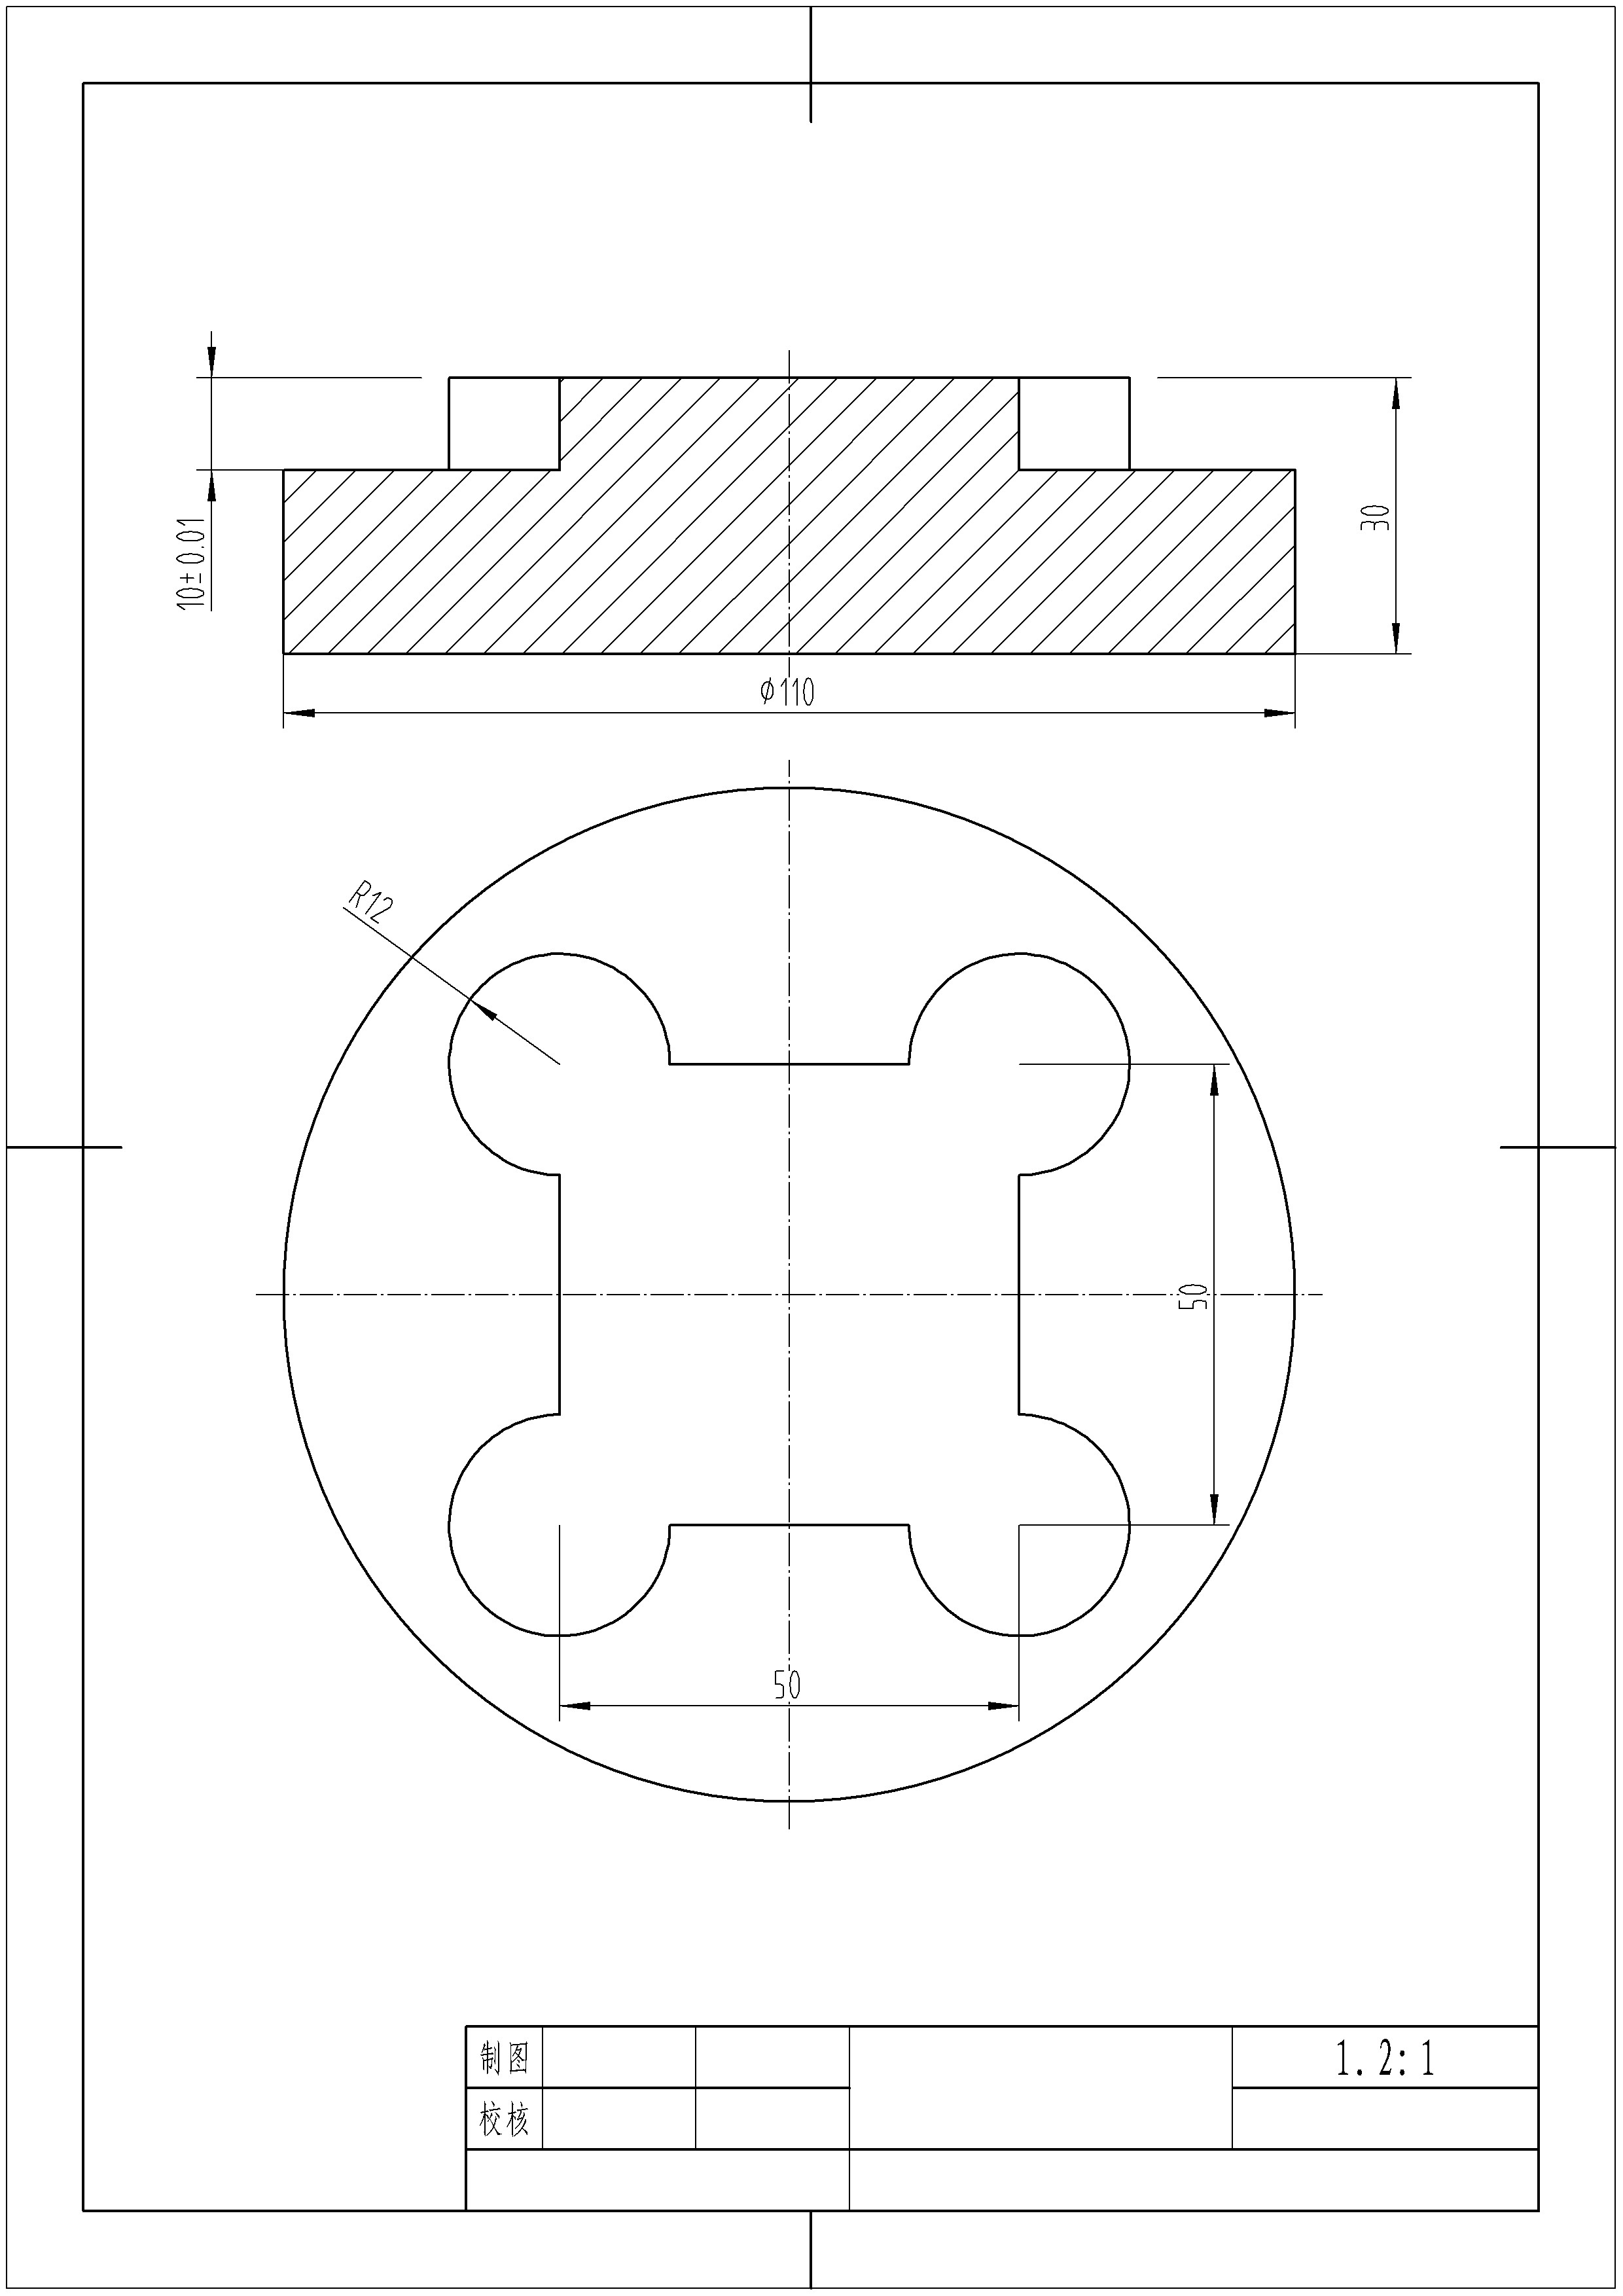
\includegraphics[width=0.8\linewidth,trim=50 150 50 100,clip]{data/image/5-2.jpg}
    \caption{}
    \label{fig:4-1}
\end{figure}

\begin{enumerate}[1、]
    \item 图样分析;
    \item 确定加工内容;
    \item 确定装夹及工件坐标系;
    \item 确定刀具及切削用量;
    \item 确定工序及走刀路线;
    \item 计算点坐标;
    \item 编写程序单。
\end{enumerate}


路径特点:

圆弧的圆心角大于180度,显然不能直接用前面的程序。

解决方法:解决方法:



1、把圆弧分成多个圆心角小于180度的圆弧。

2、掌握圆心角大于180度圆弧指令的使用。

当圆心角大于180度时,用负的半径值来表示。

当圆心角小于180度时,用正的半径值来表示。

Siemens上用CR= 正负规则一样。



\subsubsection{整圆编程}
在数控铣床或加工中心上用整圆的路径进行面铣,面铣深度为1mm,试完成加工成型的编写。
\begin{figure}[h]
    \centering
    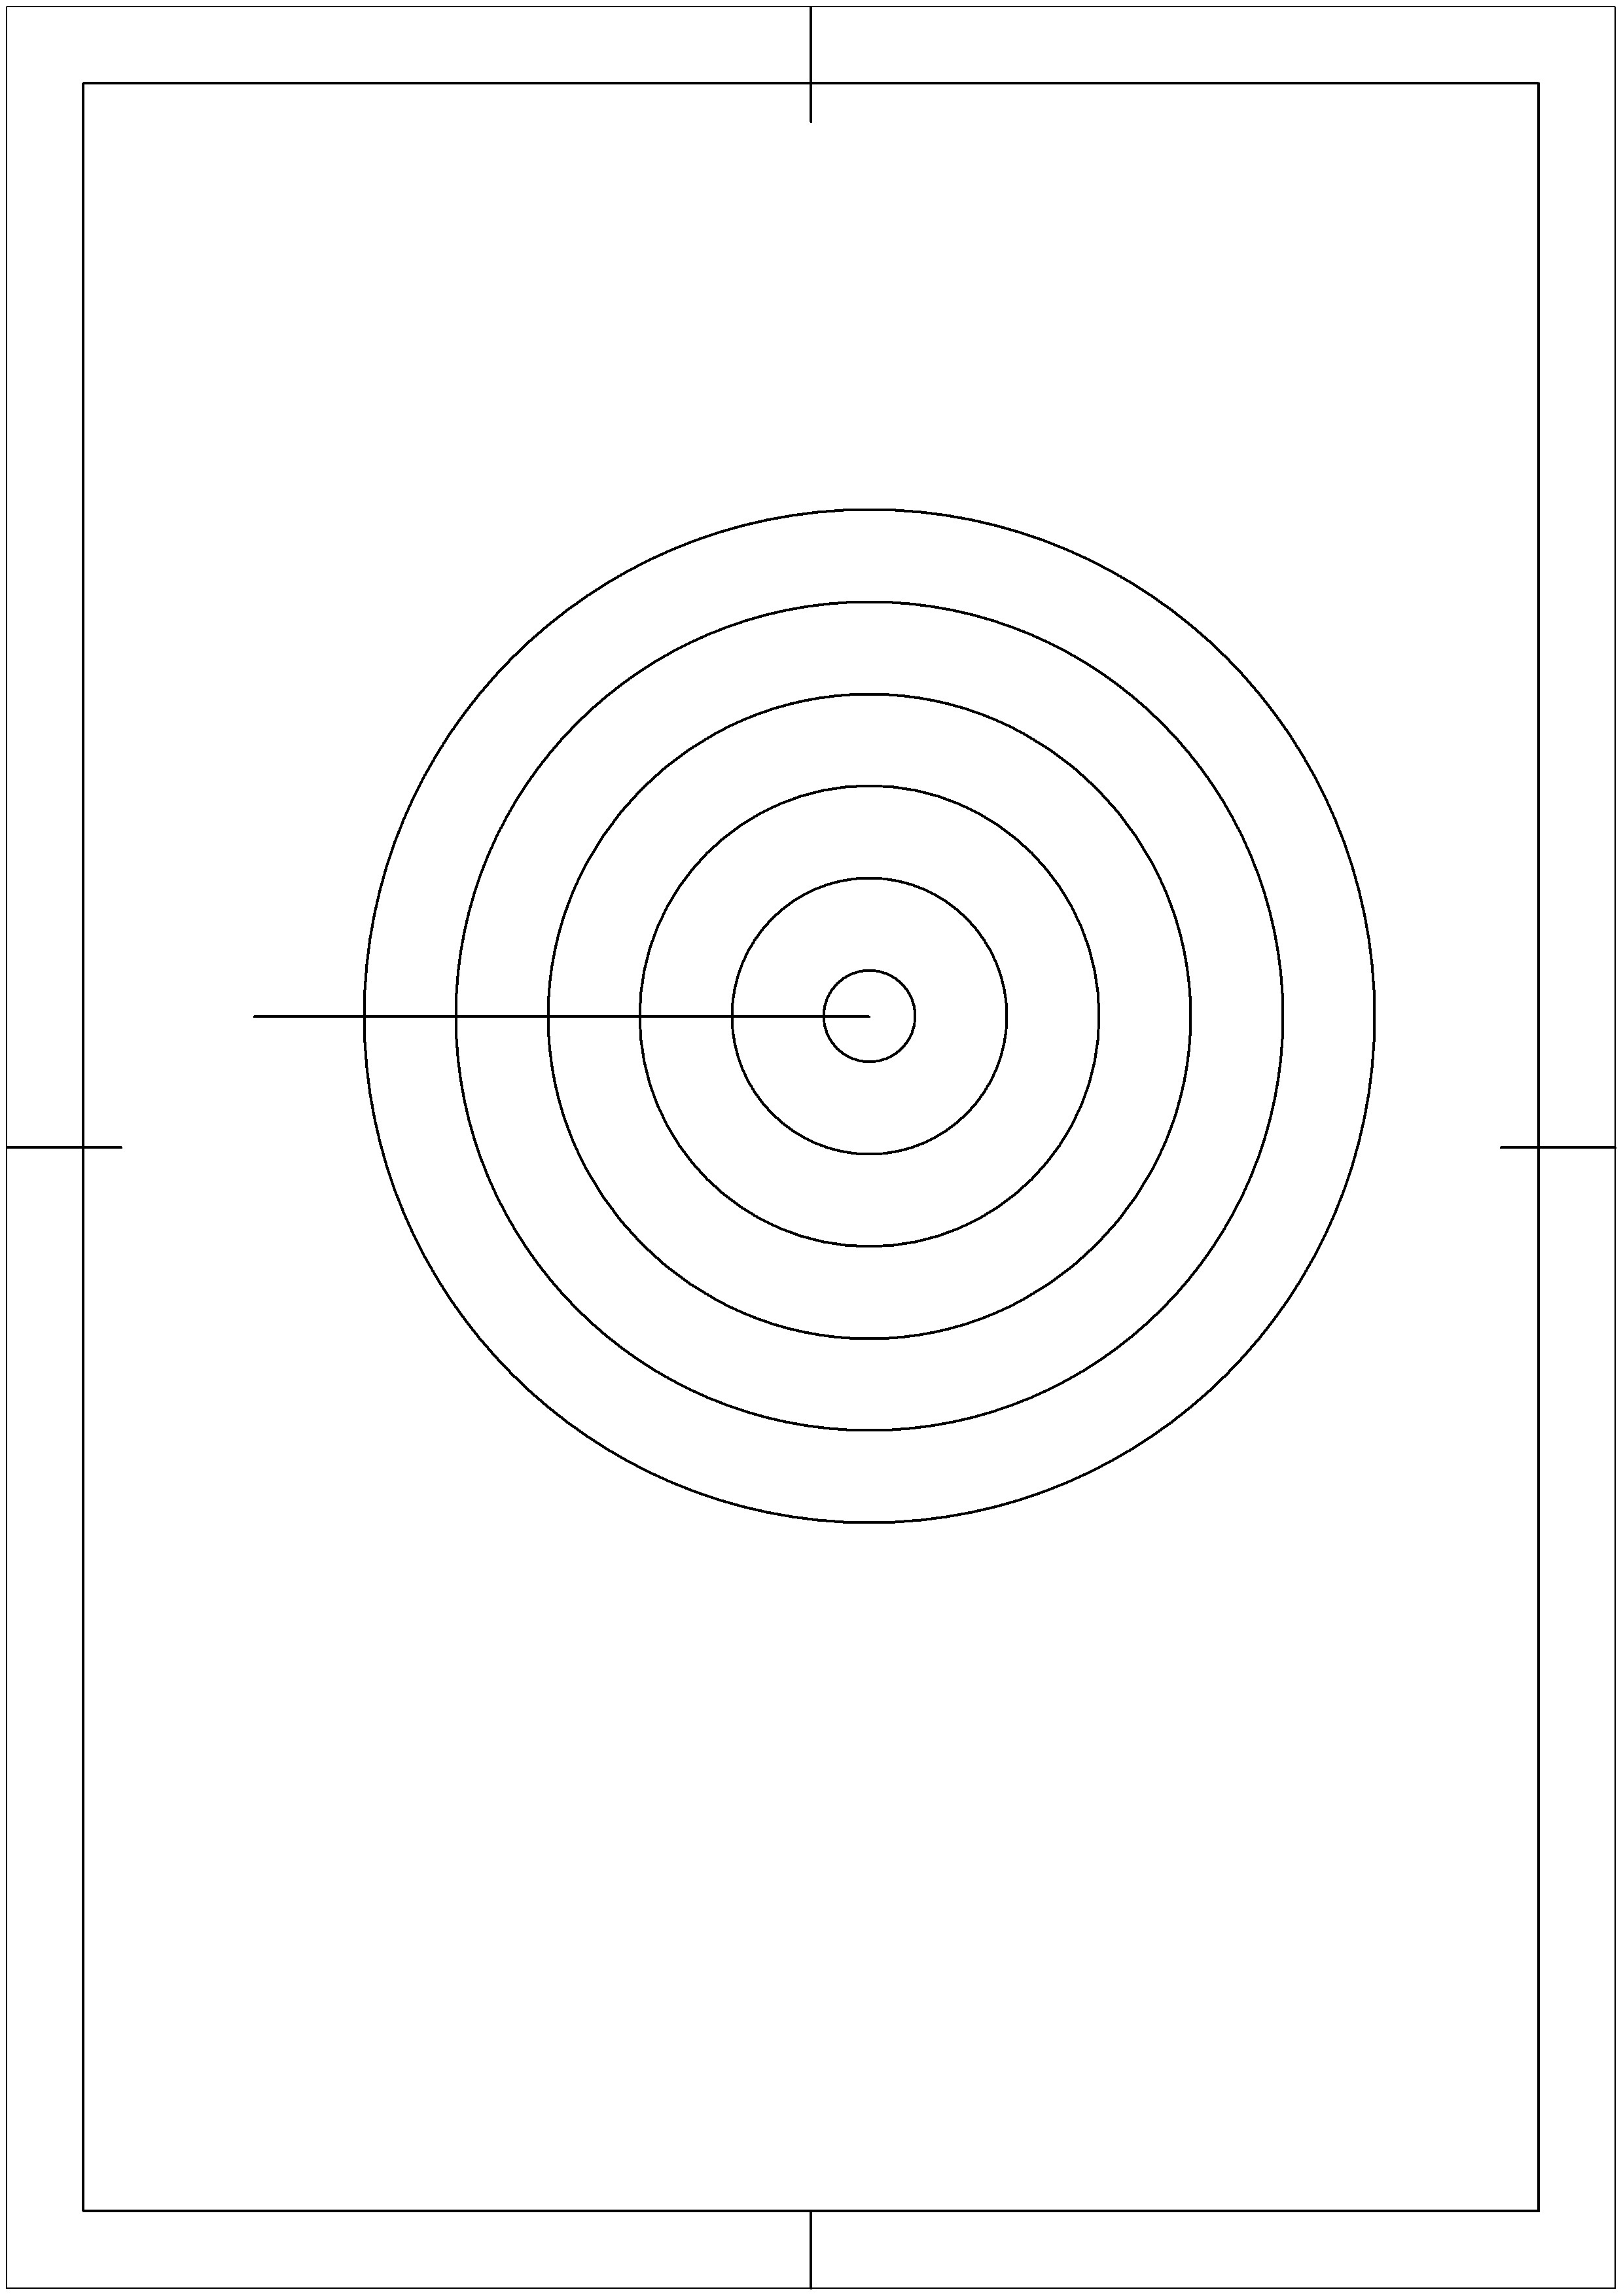
\includegraphics[width=0.8\linewidth,trim=50 150 50 100,clip]{data/image/5-3.jpg}
    \caption{}
    \label{fig:5-3}
\end{figure}

整圆路径也可以分成多个圆弧。

一个整圆路径可以用IJK圆心来编程。

不能用半径来编写一个整圆。


I、J、K表示圆心相对于起点的坐标。即:

I=X圆心-X起点

J=Y圆心-Y起点

K=Z圆心-Z起点

I、J、K与G90/G91无关,只与整圆的起点有关。

如: G17 G90 G2 X-50.0 Y-50.0 I50.0 J0;

参考程序:

\begin{lstlisting}
O0001;
G54G17G90;
M3S500;
G1Z30.0F2000;
X-65.Y0;
Z5.0;
Z-1.0F200;
X-55.0;
G2X-55.0Y0I55.0;
G1X-45.0;
G2I45.0;
G1X-35.0;
G2I-35.0;
G1X-25.0;
G2I-25.0;
G1X-15.0;
G2I-15.0;
G1X-5.0;
G2I5.0;
G1Z5.0;
Z30.0F2000;
M5;
M30;
\end{lstlisting}

\subsubsection{I、J、K的应用}
在数控铣床或加工中心上加工如图所示的零件,试用I、J、K完成程序的编写。
\begin{figure}[h]
    \centering
    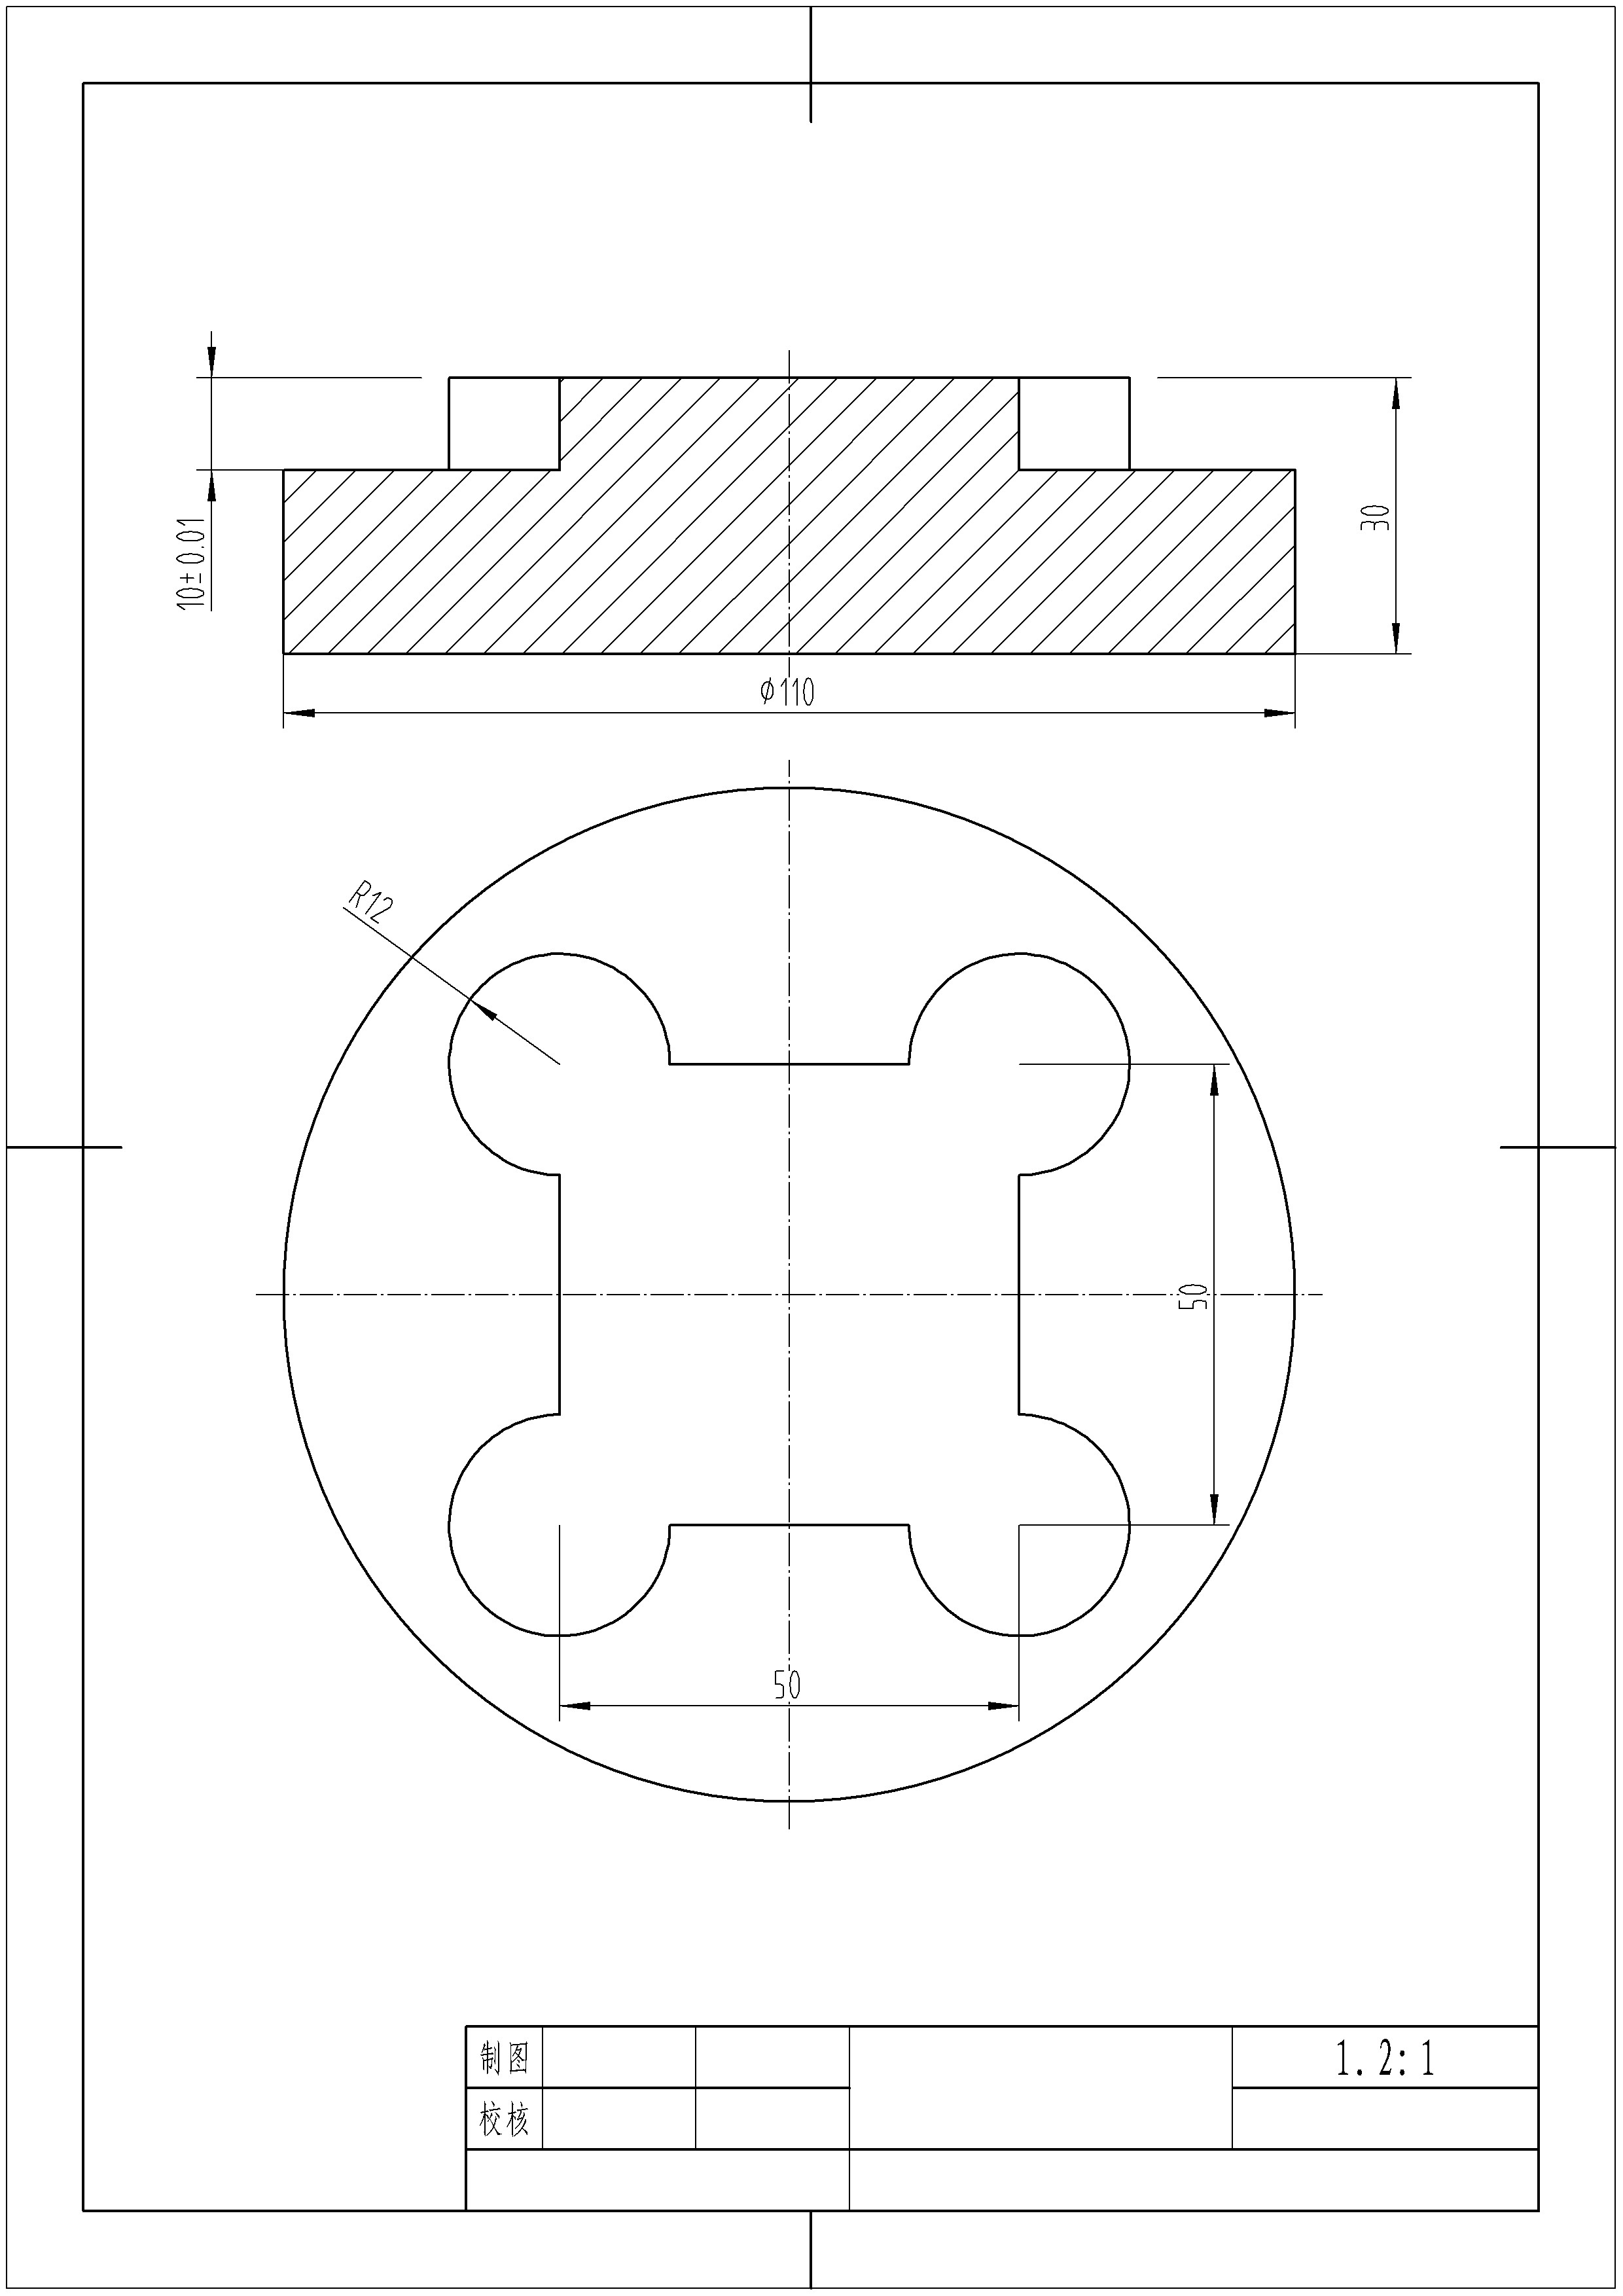
\includegraphics[width=0.8\linewidth,trim=50 150 50 100,clip]{data/image/5-4.jpg}
    \caption{}
    \label{fig:5-4}
\end{figure}
参考程序:

\begin{lstlisting}
O0001;
G54G17G90;
M3S500;
G1Z30.0F2000;
X-65.0Y0;
Z5.0;
Z-10.0F2000;
X-25.0;
Y13.0;
G2X-13.0Y25.0J13.0;
G1X13.0;
G2X25.0Y13.OJ-13.0;
….
\end{lstlisting}






手工编程中,能用半径编程就用半径编程,一般零件图标的是半径,也不容易出错。

自动编程,可以输出I、J、K以增加程序在不同机床通用性。


\subsubsection{编写程序的基本思路}
程序初始化(安全保护)--------辅助准备(换刀,主轴启动,切削液开)--------定位到起刀点--------快速下刀--------工进下刀--------走加工轮廓--------提刀---------快速提刀到安全平面-------程序结束(换刀,主轴停止,切削液关,程序返回等)
\subsection{课堂小结}
\begin{enumerate}[1、]
\item 案例分析;
\item 指令讲解;
\item 编写程序;
\item 编写程序的基本思路。
\end{enumerate}
\vfill
\subsection{布置作业}
\begin{enumerate}[1、]
	\item 自定尺寸,编写加工一个矩形外形的程序?
\end{enumerate}
\vfill